\subsection{Types of RF interface}
In ISO/IEC 14443-2 describes two types of RF interface about contactless IC cards which operate at 13.56 MHz: Type A and Type B. 

In Type A, the signal from PCD (Proximity Coupling Device) to PICC (Proximity Integrated Circuit Device) is modulated in ASK (Amplitude Shift Keying) with modulation index 100\%. When receiving the data from PCD, the PICC can’t process the data because the absence of the clock source. 

In Type B,  the signal from PCD to PICC is defined to be modulated with BPSK by carrier, and the signal from PCD to PICC is modulated in ASK with modulation index 10\%, which make it possible for PICC to work continuously. Therefore, the solution given by Type B could reach higher data rate, but the design of the circuits would be more complicated. The ASK index 10\% is harder to detect than index 100\%.

This paper describes the circuit design for the Type A. 


\subsection{Analog Front-End Modules}

The contactless IC card contains two main sections: RF section and Data Processing Unit (DPU). The modules in RF section are demonstrated in Fig.\ref{fig:modules}, which comprises Power Supply Generator (PSG), Clock Generator (CG), Voltage Regulator (VR), Power On Reset (POR), Modulator  and Demodulator. 

\begin{figure}[]
  \centering
  \includegraphics[page=9,width=80mm]{images-crop.pdf}
  \caption{Contactless IC card modules}
  \label{fig:modules}
\end{figure}

When the PICC enters to the RF field, the signal coupled by antenna can generate power supply through PSG. The PSG consists of a rectifier and a Shunt Regulator. The VG regulates the power of PSG and gives a constant voltage to the rest of the modules. As soon as the power supply reaches the operating condition, the POR gives a low level signal to reset all the Flip-Flops of the DPU. The modulator and demodulator are modules that let the PCD communicate with PICC.